\chapter{Cơ sở lý thuyết: Phát hiện và theo dõi đối tượng}
\label{ch:ly_thuyet_detection}

\section{Tổng quan về bài toán Phát hiện đối tượng}

\subsection{Giới thiệu chung}
Phát hiện đối tượng (Object Detection) là một bài toán nền tảng và thiết yếu trong lĩnh vực Thị giác máy tính (Computer Vision). Mục đích chính của bài toán là xác định sự hiện diện của các thực thể quan tâm trong một hình ảnh kỹ thuật số hoặc video, đồng thời định vị chính xác vị trí và gán nhãn phân loại cho từng thực thể đó.

Khác với bài toán phân loại ảnh (Image Classification) đơn thuần chỉ gán một nhãn duy nhất cho toàn bộ bức ảnh, phát hiện đối tượng giải quyết đồng thời hai nhiệm vụ phức tạp:
\begin{enumerate}
    \item \textbf{Định vị (Localization):} Xác định vị trí của đối tượng thông qua một khung bao (Bounding Box).
    \item \textbf{Phân loại (Classification):} Xác định danh mục (class) của đối tượng nằm trong khung bao đó.
\end{enumerate}

Bài toán này đóng vai trò tiền đề cho nhiều ứng dụng thực tế quan trọng như: xe tự hành (autonomous driving), hệ thống giám sát an ninh, chẩn đoán y tế qua hình ảnh và tương tác người-máy.

\subsection{Định nghĩa toán học}
Về mặt hình thức, xét một ảnh đầu vào $I \in \mathbb{R}^{H \times W \times C}$, trong đó $H, W, C$ lần lượt là chiều cao, chiều rộng và số kênh màu của ảnh. Mục tiêu của mô hình $f(I)$ là dự đoán một tập hợp các bounding box $B = \{b_1, b_2, \dots, b_N\}$, trong đó mỗi $b_i$ đại diện cho một đối tượng được phát hiện và được định nghĩa bởi vector:
\begin{equation}
    b_i = (x_i, y_i, w_i, h_i, c_i, p_i)
\end{equation}

Các tham số được giải thích cụ thể như sau:
\begin{itemize}
    \item $(x_i, y_i)$: Tọa độ tâm của bounding box, thường được chuẩn hóa theo kích thước ảnh hoặc so với lưới đặc trưng (feature grid).
    \item $(w_i, h_i)$: Chiều rộng và chiều cao của bounding box. Trong các mô hình hiện đại, giá trị này thường được dự đoán dưới dạng độ lệch (offset) log-space so với các khung neo (anchor) định trước.
    \item $c_i \in \{1, \dots, K\}$: Nhãn lớp của đối tượng, thuộc một trong $K$ danh mục quan tâm (ví dụ: người, xe, chó, mèo).
    \item $p_i \in [0, 1]$: Độ tin cậy (confidence score), phản ánh xác suất mà mô hình tin rằng bounding box này chứa một đối tượng thực sự thuộc lớp $c_i$.
\end{itemize}

\subsection{Thách thức của bài toán}
Việc ánh xạ từ không gian pixel sang không gian ngữ nghĩa của các bounding box gặp phải nhiều thách thức lớn, bao gồm:
\begin{itemize}
    \item \textbf{Sự biến thiên về tỷ lệ (Scale Variation):} Các đối tượng trong ảnh có thể xuất hiện với kích thước rất khác nhau, từ vài pixel đến chiếm toàn bộ khung hình.
    \item \textbf{Sự che khuất (Occlusion):} Các đối tượng có thể bị che khuất một phần bởi các đối tượng khác hoặc nền, làm mất đi các đặc trưng quan trọng để nhận dạng.
    \item \textbf{Điều kiện ánh sáng:} Sự thay đổi về ánh sáng, bóng đổ, phản chiếu ảnh hưởng đến chất lượng ảnh đầu vào.
    \item \textbf{Giao thông hỗn hợp:} Đặc thù tại Việt Nam với nhiều loại phương tiện di chuyển xen kẽ nhau.
\end{itemize}


\section{Cơ sở lý thuyết về mô hình YOLO}

\subsection{Hợp nhất bài toán thành một mạng duy nhất}
Trước khi kiến trúc YOLO (You Only Look Once) ra đời, các hệ thống phát hiện đối tượng kinh điển thường xử lý bài toán theo quy trình hai giai đoạn tách biệt (Two-Stage Detectors). Các phương pháp như R-CNN sử dụng thuật toán đề xuất vùng (Region Proposal) như Selective Search để tìm kiếm các vùng ứng viên, sau đó mới áp dụng bộ phân loại trên từng vùng này. Quy trình này tốn kém về mặt tính toán và khó tối ưu hóa toàn cục.

YOLO, được giới thiệu bởi Redmon et al. (2015), đã thay đổi hoàn toàn tư duy này bằng cách tái định nghĩa việc phát hiện đối tượng thành một bài toán \textbf{hồi quy duy nhất} (Single Regression Problem). Thay vì quét ảnh nhiều lần, YOLO chỉ cần một lần truyền thẳng (forward pass) qua mạng nơ-ron tích chập (CNN) để dự đoán đồng thời cả vị trí khung bao (bounding box) và xác suất lớp đối tượng. Điều này cho phép mô hình nhìn thấy ngữ cảnh toàn cục của bức ảnh, giảm thiểu các sai sót do nhầm lẫn hậu cảnh (background).

\subsection{Cơ chế chia lưới và Biểu diễn đầu ra}

Cơ chế hoạt động cốt lõi của mọi phiên bản YOLO dựa trên việc chia ảnh đầu vào thành một lưới kích thước $S \times S$. Quy tắc gán nhãn được định nghĩa như sau:
\begin{itemize}
    \item Nếu tâm (center) của một đối tượng thực tế rơi vào ô lưới nào, ô lưới đó chịu trách nhiệm phát hiện đối tượng đó.
    \item Mỗi ô lưới sẽ dự đoán $B$ khung bao dự kiến, cùng với độ tin cậy (confidence) cho mỗi khung bao.
\end{itemize}

Về mặt toán học, độ tin cậy $C_{pred}$ được định nghĩa là tích của xác suất có đối tượng và độ chồng lấn (IoU) với thực tế:
\begin{equation}
    C_{pred} = Pr(\text{Object}) \times \text{IoU}_{pred}^{truth}
\end{equation}
Nếu không có đối tượng trong ô lưới, $Pr(\text{Object}) = 0$, dẫn đến $C_{pred} = 0$.

Đầu ra của mạng là một tensor 3 chiều có kích thước $S \times S \times (B \times 5 + K)$, trong đó $K$ là số lớp đối tượng. Mỗi vector dự đoán bao gồm 5 tham số cơ bản:
\begin{equation}
    \hat{y} = (t_x, t_y, t_w, t_h, t_o)
\end{equation}
Trong đó $(t_x, t_y)$ là tọa độ tâm cục bộ trong ô lưới, $(t_w, t_h)$ là kích thước khung bao được chuẩn hóa, và $t_o$ là độ tin cậy.

\begin{figure}[!htbp]
    \centering
    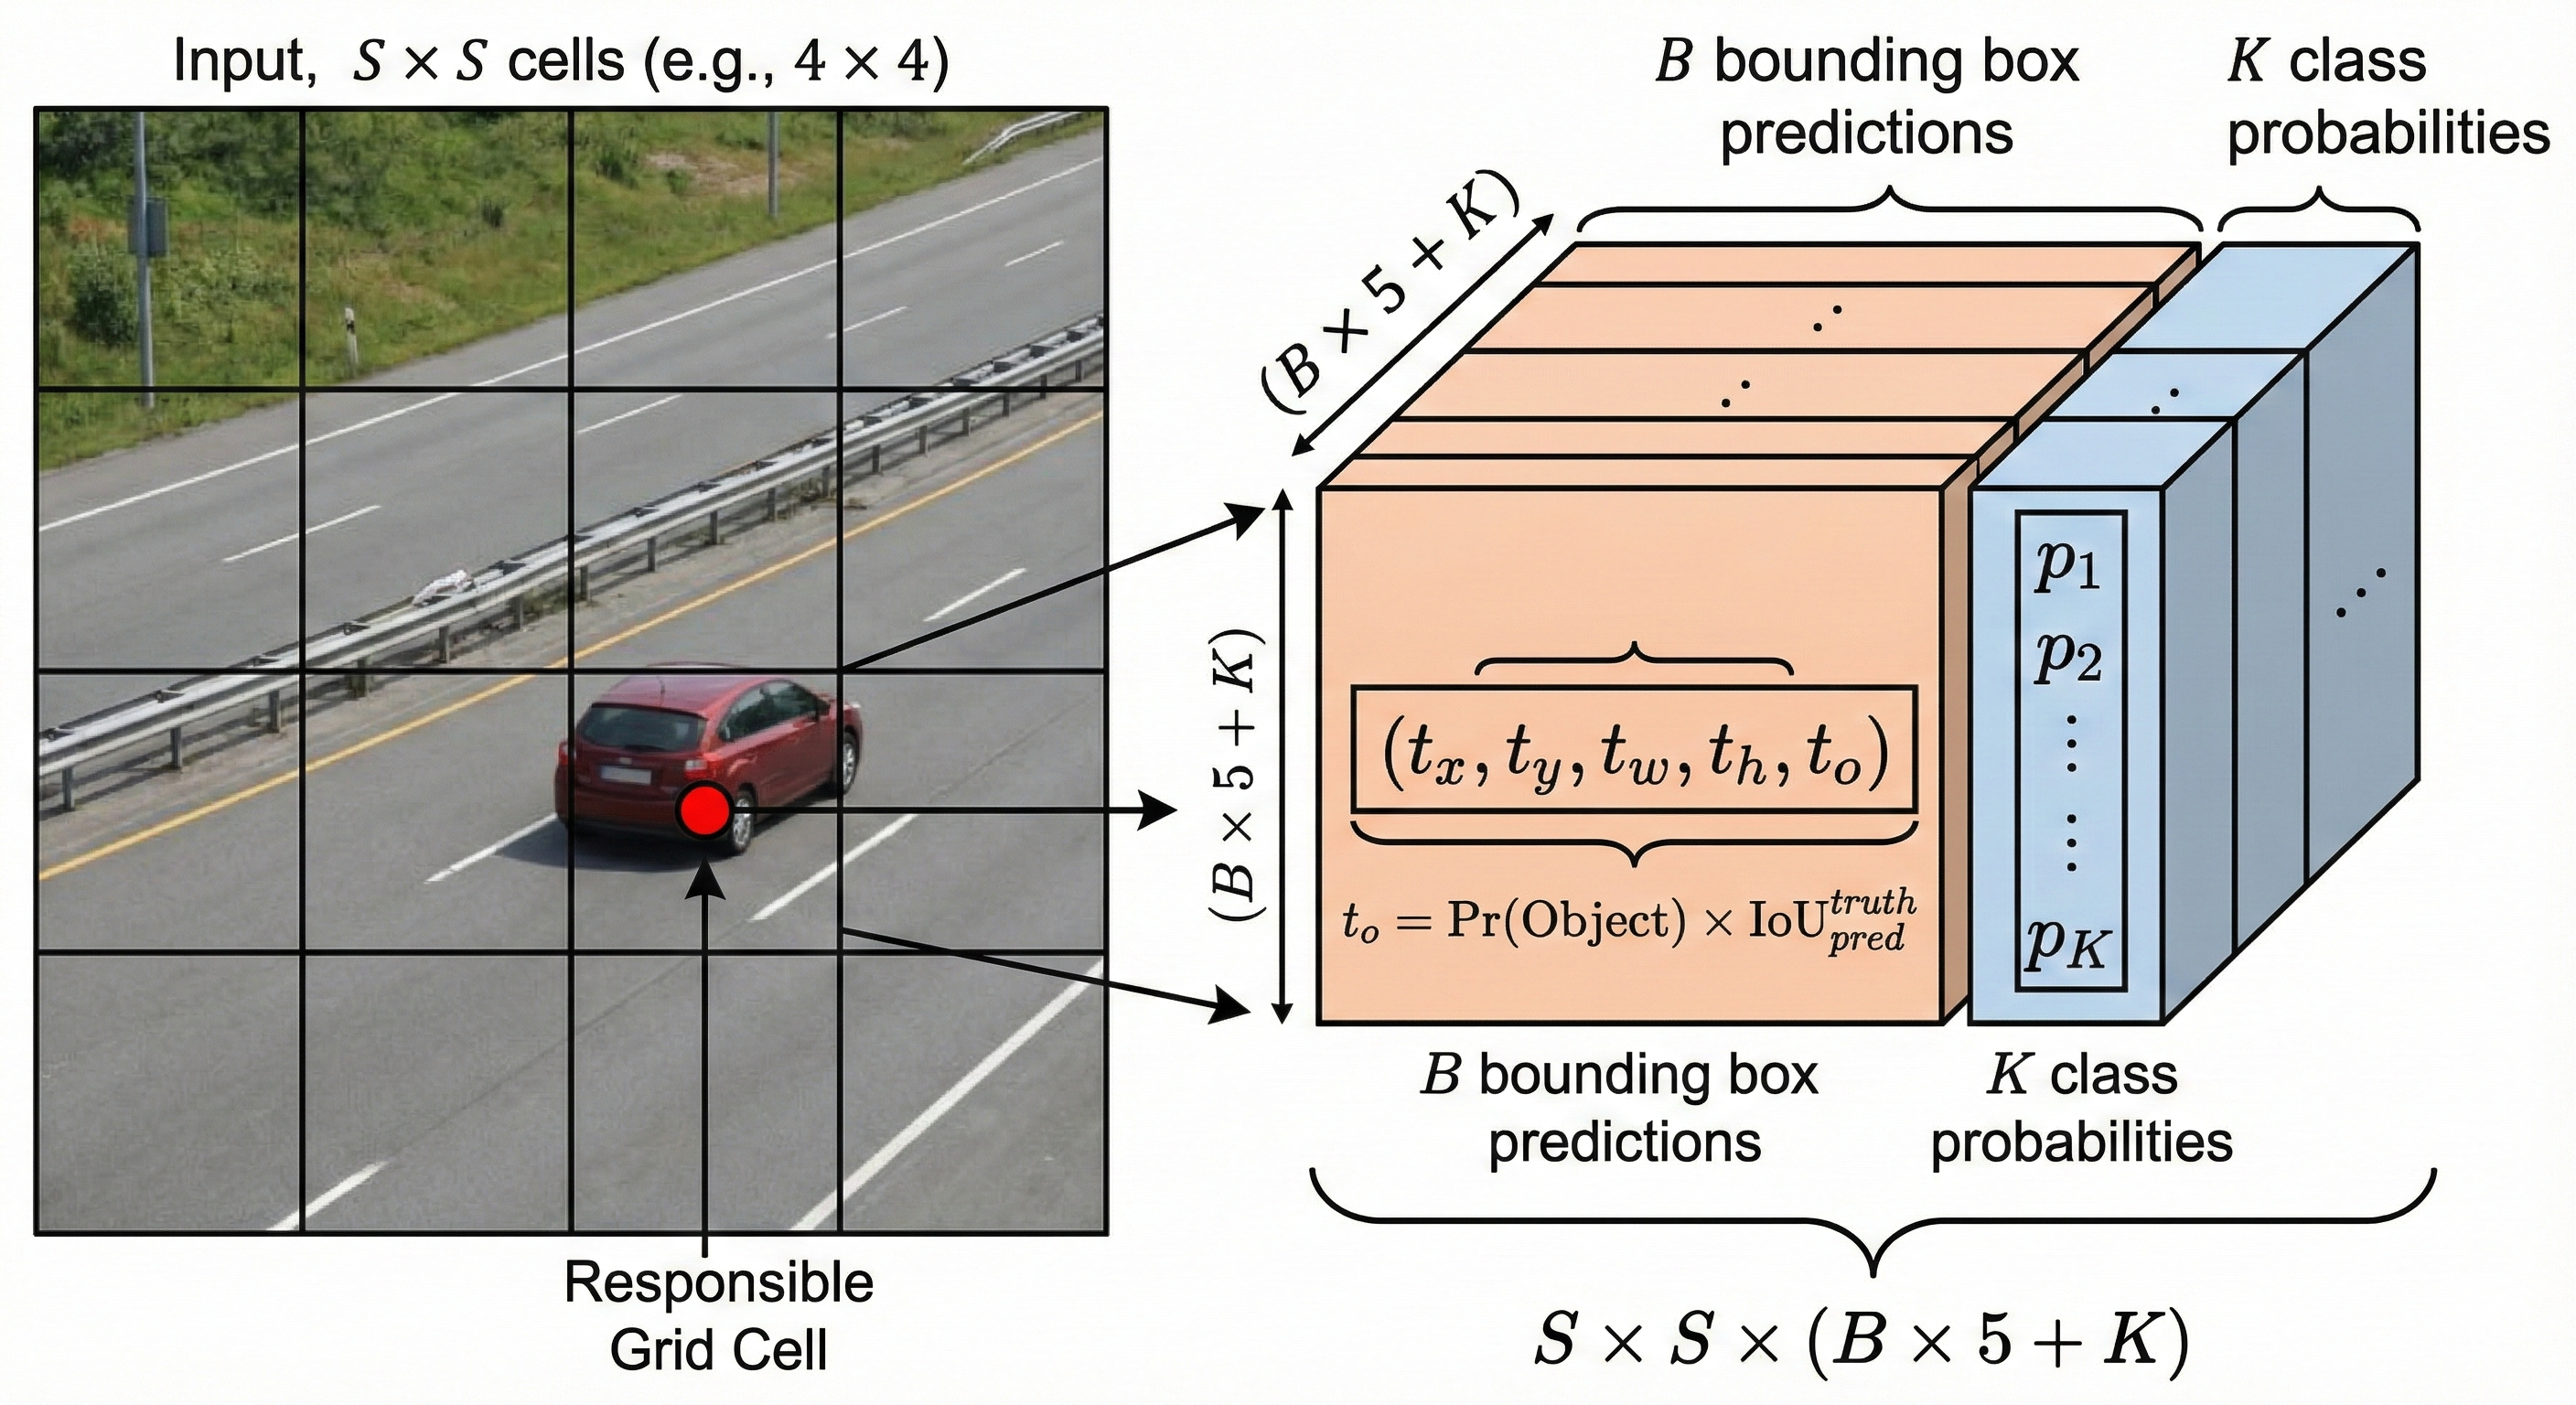
\includegraphics[width=0.8\linewidth]{Figures/chia_luoi.png}
    \caption{Cơ chế chia lưới và biểu diễn đầu ra của YOLO}
    \label{fig:grid_yolo}
\end{figure}

\subsection{Kiến trúc mạng tổng quát}

Hầu hết các phiên bản YOLO hiện đại đều tuân theo kiến trúc Meta-architecture gồm 3 thành phần chính:
\begin{enumerate}
    \item \textbf{Backbone (Xương sống):} Là một mạng CNN đóng vai trò trích xuất đặc trưng từ ảnh đầu vào ở các mức độ phân giải khác nhau.
    \item \textbf{Neck (Cổ):} Sử dụng các kỹ thuật như Feature Pyramid Network (FPN) hoặc Path Aggregation Network (PANet) để trộn và kết hợp các đặc trưng từ Backbone, giúp mô hình nhận diện tốt cả đối tượng nhỏ và lớn.
    \item \textbf{Head (Đầu):} Thực hiện nhiệm vụ cuối cùng là dự đoán lớp và tọa độ khung bao trên các bản đồ đặc trưng đã được tổng hợp.
\end{enumerate}

\subsection{Sự tiến hóa và Lựa chọn YOLOv8}
Trải qua quá trình phát triển, YOLO đã có những bước tiến vượt bậc:
\begin{itemize}
    \item \textbf{YOLOv1-v3:} Tập trung vào triển khai thời gian thực, giới thiệu khái niệm Anchor Box để ổn định việc huấn luyện.
    \item \textbf{YOLOv4-v5:} Tối ưu hóa mạnh mẽ về kỹ thuật huấn luyện (Training Tricks) như Mosaic Augmentation và cải tiến kiến trúc với CSPNet để tăng cường luồng gradient.
    \item \textbf{YOLOv6-v8 (2022-2023):} Đánh dấu sự chuyển dịch sang kiến trúc \textbf{Anchor-free} (không dùng khung neo) và \textbf{Decoupled Head} (tách riêng nhánh phân loại và hồi quy).
\end{itemize}

\textbf{Lý do lựa chọn YOLOv8:}
Đề tài này lựa chọn \textbf{YOLOv8} (Ultralytics, 2023) làm mô hình chủ đạo. Đây là phiên bản không quá nặng, kế thừa tinh hoa của các thế hệ trước nhưng sở hữu các cải tiến vượt trội phù hợp cho bài toán giao thông tại Việt Nam:
\begin{itemize}
    \item \textbf{Anchor-free:} Loại bỏ nhu cầu thiết kế kích thước anchor box thủ công, giúp mô hình linh hoạt hơn với các đối tượng có tỷ lệ kích thước biến thiên lớn (như xe máy chở hàng cồng kềnh, xe buýt).
    \item \textbf{C2f Module:} Thay thế module C3 cũ, giúp mô hình nhẹ hơn nhưng trích xuất đặc trưng phong phú hơn nhờ các luồng gradient song song.
    \item \textbf{Task Aligned Assigner:} Cơ chế gán nhãn động thông minh, giúp cân bằng tốt hơn giữa mẫu dương và mẫu âm trong quá trình huấn luyện.
\end{itemize}

\section{Mô hình YOLOv8 chi tiết}
YOLOv8 là mô hình phát hiện đối tượng một giai đoạn (one-stage detector) tiên tiến, coi bài toán phát hiện đối tượng là một bài toán hồi quy trực tiếp từ các pixel của ảnh sang tọa độ bounding box và xác suất lớp.

\subsection{Cơ chế Anchor-free}
Khác với các thế hệ trước dựa trên Anchor Box (khung neo), YOLOv8 áp dụng phương pháp \textbf{Anchor-free}. Thay vì dự đoán độ lệch (offset) so với anchor box, mô hình dự đoán trực tiếp khoảng cách từ tâm của ô lưới (grid cell) đến 4 cạnh của bounding box thực tế.

Giả sử tâm của một đối tượng rơi vào ô lưới tại tọa độ $(c_x, c_y)$, mô hình sẽ dự đoán vector 4 chiều $t = (l, t, r, b)$ đại diện cho khoảng cách tới cạnh trái, trên, phải, và dưới.

\subsection{Các thành phần kiến trúc đặc trưng}

\subsubsection{Module C2f (Cross Stage Partial with 2 flow)}
YOLOv8 giới thiệu module C2f để thay thế cho module C3 trong các phiên bản trước. C2f được thiết kế dựa trên ý tưởng của kiến trúc ELAN (Efficient Layer Aggregation Network), giúp cải thiện luồng gradient thông tin trong mạng nơ-ron mà không làm tăng đáng kể chi phí tính toán.

Cơ chế hoạt động của C2f bao gồm hai bước:
\begin{enumerate}
    \item Tách tensor đầu vào thành hai phần theo kênh (channel-wise split).
    \item Một phần đi qua chuỗi các lớp Bottleneck, phần còn lại đi thẳng (shortcut). Cuối cùng, tất cả các nhánh được nối (concatenate) lại với nhau.
\end{enumerate}

Công thức tổng quát cho đầu ra $Y$ của khối C2f có thể mô tả như sau:
\begin{equation}
    Y = \text{Conv}_{1\times1}([X_1, \text{Block}_1(X_2), \text{Block}_2(\text{Block}_1(X_2)), \dots])
\end{equation}

Kiến trúc này giúp mô hình học được các đặc trưng phong phú hơn (richer features) nhờ việc kết hợp thông tin ở nhiều độ sâu khác nhau.

\subsubsection{Module SPPF (Spatial Pyramid Pooling Fast)}
Nằm ở cuối phần Backbone, module SPPF có nhiệm vụ trích xuất các đặc trưng ngữ cảnh không gian (spatial context features) ở nhiều tỷ lệ khác nhau. Thay vì sử dụng các bộ lọc có kích thước lớn gây tốn kém tính toán, SPPF thực hiện tuần tự 3 lần phép gộp cực đại (Max Pooling) với kích thước $5 \times 5$.

Đầu ra là sự kết hợp (concatenation) của đầu vào gốc và đầu ra của 3 lần pooling:
\begin{equation}
    \text{Out} = \text{Concat}(X, \text{MaxPool}(X), \text{MaxPool}^2(X), \text{MaxPool}^3(X))
\end{equation}

Điều này giúp mô hình nhận diện tốt các đối tượng có kích thước thay đổi lớn (như xe buýt so với xe máy) và thuận lợi cho triển khai.

\subsubsection{Chiến lược gán nhãn Task Aligned Assigner}
Một trong những cải tiến quan trọng nhất của YOLOv8 là loại bỏ cơ chế gán nhãn dựa trên IoU tĩnh (static IoU-based assignment) và thay thế bằng \textbf{Task Aligned Assigner}. Chiến lược này chọn lọc các mẫu dương (positive samples) dựa trên sự cân bằng giữa điểm phân loại và chất lượng định vị.

Điểm số căn chỉnh (alignment score) $t$ cho mỗi anchor point được tính như sau:
\begin{equation}
    t = s^\alpha \times u^\beta
\end{equation}
Trong đó:
\begin{itemize}
    \item $s$: Điểm số phân loại dự đoán (predicted classification score).
    \item $u$: Chỉ số IoU giữa box dự đoán và box thực tế.
    \item $\alpha$ và $\beta$: Các tham số điều trọng số (thường $\alpha=0.5, \beta=6.0$).
\end{itemize}

Chỉ những mẫu có điểm $t$ cao nhất mới được chọn làm mẫu dương để huấn luyện. Cơ chế này giúp mô hình tập trung vào các dự đoán chất lượng cao, nơi mà "phân loại đúng" đi đôi với "định vị chính xác".

\subsection{Hàm mất mát (Loss Function)}
Quá trình huấn luyện YOLOv8 nhằm tối thiểu hóa hàm mất mát tổng hợp $L_{total}$, bao gồm hai thành phần chính: mất mát về định vị ($L_{box}$) và mất mát về phân loại ($L_{cls}$).
\begin{equation}
    L_{total} = \lambda_{box} L_{box} + \lambda_{cls} L_{cls} + \lambda_{dfl} L_{dfl}
\end{equation}

\subsubsection{Mất mát định vị (Box Loss)}
YOLOv8 sử dụng hàm mất mát \textbf{CIoU (Complete IoU)} để đo lường sai số giữa khung dự đoán ($B_{pred}$) và khung thực tế ($B_{gt}$). CIoU khắc phục nhược điểm của IoU truyền thống bằng cách xem xét thêm khoảng cách tâm và tỷ lệ khung hình.

Công thức CIoU được định nghĩa như sau:
\begin{equation}
    \mathcal{L}_{CIoU} = 1 - IoU + \frac{\rho^2(\mathbf{b}, \mathbf{b}^{gt})}{c^2} + \alpha v
\end{equation}
Trong đó:
\begin{itemize}
    \item $IoU = \frac{|B_{pred} \cap B_{gt}|}{|B_{pred} \cup B_{gt}|}$ là chỉ số giao trên hợp.
    \item $\rho(\cdot)$ là khoảng cách Euclidean giữa tâm của hai bounding box $\mathbf{b}$ và $\mathbf{b}^{gt}$.
    \item $c$ là đường chéo của bao lồi nhỏ nhất chứa cả hai box.
    \item $\alpha$ là tham số cân bằng trọng số.
    \item $v$ đo lường sự tương đồng về tỷ lệ khung hình (aspect ratio consistency):
    \begin{equation}
        v = \frac{4}{\pi^2} \left( \arctan\frac{w^{gt}}{h^{gt}} - \arctan\frac{w}{h} \right)^2
    \end{equation}
\end{itemize}

Ngoài ra, YOLOv8 còn kết hợp \textbf{Distribution Focal Loss (DFL)} để tối ưu hóa phân phối xác suất của các cạnh bounding box, giúp mô hình hội tụ ổn định hơn khi dự đoán các box có biên mờ.

\subsubsection{Mất mát phân loại (Classification Loss)}
Đối với nhánh phân loại, YOLOv8 sử dụng \textbf{Varifocal Loss (VFL)} hoặc Binary Cross Entropy (BCE). VFL giúp cân bằng giữa các mẫu dương (positive samples) và mẫu âm (negative samples) khó học:
\begin{equation}
    VFL(p, q) = \begin{cases}
    -q (q \log(p) + (1-q) \log(1-p)) & \text{nếu } q > 0 \\
    -\alpha p^\gamma \log(1-p) & \text{nếu } q = 0
    \end{cases}
\end{equation}
Trong đó $p$ là xác suất dự đoán và $q$ là điểm IoU mục tiêu (target IoU score).

\section{Theo dõi đa đối tượng (Multi-Object Tracking)}
\label{sec:tracking_theory}

Bài toán Theo dõi đa đối tượng (Multi-Object Tracking - MOT) nhằm mục đích ước lượng quỹ đạo của các đối tượng trong video. Giả sử tại mỗi khung hình $t$, ta nhận được một tập hợp các detection $D_t = \{d_1, d_2, \dots, d_n\}$. Mục tiêu là gán một ID duy nhất $k$ cho mỗi chuỗi detection $(d_{t_1}^k, d_{t_2}^k, \dots)$ tương ứng với cùng một thực thể thực tế.

Hệ thống sử dụng phương pháp \textbf{Tracking-by-Detection} kết hợp với thuật toán \textbf{ByteTrack}, trong đó thành phần cốt lõi là Bộ lọc Kalman để ước lượng trạng thái và thuật toán Hungarian để liên kết dữ liệu.

\subsection{Bộ lọc Kalman (Kalman Filter)}
Bộ lọc Kalman là một thuật toán đệ quy tối ưu để ước lượng trạng thái của một hệ thống động lực học từ các phép đo nhiễu. Trong bài toán tracking phương tiện, chúng tôi mô hình hóa chuyển động của xe là chuyển động đều (constant velocity model).

\subsubsection{Không gian trạng thái (State Space)}
Trạng thái của một phương tiện tại thời điểm $k$ được biểu diễn bởi vector 8 chiều $\mathbf{x}_k$:
\begin{equation}
    \mathbf{x}_k = [u_k, v_k, a_k, h_k, \dot{u}_k, \dot{v}_k, \dot{a}_k, \dot{h}_k]^T
\end{equation}
Trong đó:
\begin{itemize}
    \item $(u_k, v_k)$: Tọa độ tâm của bounding box.
    \item $a_k$: Tỷ lệ khung hình (aspect ratio $w/h$).
    \item $h_k$: Chiều cao của bounding box.
    \item $\dot{u}_k, \dot{v}_k, \dot{a}_k, \dot{h}_k$: Vận tốc biến thiên tương ứng của các tham số trên.
\end{itemize}

\subsubsection{Quá trình Dự đoán (Prediction)}
Dựa trên trạng thái ở thời điểm trước đó $k-1$, bộ lọc dự đoán trạng thái tiên nghiệm (a priori) tại thời điểm $k$:
\begin{equation}
    \hat{\mathbf{x}}_{k|k-1} = \mathbf{F}_k \hat{\mathbf{x}}_{k-1|k-1}
\end{equation}
\begin{equation}
    \mathbf{P}_{k|k-1} = \mathbf{F}_k \mathbf{P}_{k-1|k-1} \mathbf{F}_k^T + \mathbf{Q}_k
\end{equation}
Trong đó:
\begin{itemize}
    \item $\mathbf{F}_k$: Ma trận chuyển trạng thái (state transition matrix), mô tả mô hình vật lý của chuyển động.
    \item $\mathbf{P}_{k|k-1}$: Ma trận hiệp phương sai sai số dự đoán.
    \item $\mathbf{Q}_k$: Ma trận hiệp phương sai nhiễu của quá trình (process noise).
\end{itemize}

\subsubsection{Quá trình Cập nhật (Update)}
Khi nhận được phép đo mới (measurement) $\mathbf{z}_k$ từ YOLOv8 (tọa độ bounding box $[u, v, a, h]^T$), bộ lọc sẽ hiệu chỉnh trạng thái dự đoán để có trạng thái hậu nghiệm (a posteriori) chính xác hơn:
\begin{equation}
    \mathbf{K}_k = \mathbf{P}_{k|k-1} \mathbf{H}_k^T (\mathbf{H}_k \mathbf{P}_{k|k-1} \mathbf{H}_k^T + \mathbf{R}_k)^{-1}
\end{equation}
\begin{equation}
    \hat{\mathbf{x}}_{k|k} = \hat{\mathbf{x}}_{k|k-1} + \mathbf{K}_k (\mathbf{z}_k - \mathbf{H}_k \hat{\mathbf{x}}_{k|k-1})
\end{equation}
Trong đó $\mathbf{K}_k$ là độ lợi Kalman (Kalman Gain), $\mathbf{H}_k$ là ma trận quan sát, và $\mathbf{R}_k$ là nhiễu đo lường.

\begin{figure}[!htbp]
    \centering
    \begin{tikzpicture}[node distance=3cm, auto]
        % Nodes (Đã thêm text width=5cm và align=center để sửa lỗi LR mode)
        \node (predict) [process, fill=blue!10, text width=5.5cm, align=center] {
            \textbf{Time Update (Dự đoán)}\\
            1. Dự đoán trạng thái $\hat{x}_{k|k-1}$\\
            2. Dự đoán hiệp phương sai $P_{k|k-1}$
        };

        \node (update) [process, fill=green!10, right of=predict, xshift=5.5cm, text width=5.5cm, align=center] {
            \textbf{Measurement Update (Cập nhật)}\\
            1. Tính Kalman Gain $K_k$\\
            2. Cập nhật trạng thái $\hat{x}_{k|k}$\\
            3. Cập nhật hiệp phương sai $P_{k|k}$
        };

        \node (delay) [decision, below of=predict, xshift=3.75cm, yshift=-1.5cm, aspect=2] {Delay $z^{-1}$};

        % Arrows
        \draw [arrow, bend left=30] (predict.east) -- node {Tiên nghiệm} (update.west);
        \draw [arrow, bend left=30] (update.south) to node [auto] {Hậu nghiệm} (delay.east);
        \draw [arrow, bend left=30] (delay.west) to node [auto] {Bước sau} (predict.south);
    \end{tikzpicture}
    \caption{Chu trình hoạt động của Bộ lọc Kalman}
    \label{fig:kalman_cycle}
\end{figure}

\subsection{Liên kết dữ liệu (Data Association)}
Liên kết dữ liệu là bước quyết định trong hệ thống theo dõi, đóng vai trò cầu nối giữa các đầu ra phát hiện rời rạc (discrete detections) và các quỹ đạo liên tục (continuous trajectories). Giả sử tại thời điểm $t$, ta có tập hợp $M$ quỹ đạo hiện hành $T = \{t_1, t_2, \dots, t_M\}$ và tập hợp $N$ đối tượng vừa được phát hiện $D = \{d_1, d_2, \dots, d_N\}$.

Bài toán đặt ra là tìm một ánh xạ ghép cặp 1-1 tối ưu giữa $T$ và $D$ sao cho tổng độ sai lệch (chi phí) là nhỏ nhất. Vấn đề này được mô hình hóa dưới dạng bài toán \textbf{Phân công Tuyến tính (Linear Assignment Problem)} trên đồ thị hai phía (bipartite graph).

Hàm mục tiêu cần tối thiểu hóa được biểu diễn như sau:
\begin{equation}
    \min \sum_{i=1}^{M} \sum_{j=1}^{N} C_{i,j} X_{i,j}
\end{equation}

Thỏa mãn các điều kiện ràng buộc:
\begin{equation}
    \begin{cases}
        \sum_{j=1}^{N} X_{i,j} \le 1, & \forall i = 1 \dots M \\
        \sum_{i=1}^{M} X_{i,j} \le 1, & \forall j = 1 \dots N \\
        X_{i,j} \in \{0, 1\}
    \end{cases}
\end{equation}

Trong đó:
\begin{itemize}
    \item $X_{i,j}$ là biến quyết định nhị phân: $X_{i,j} = 1$ nếu quỹ đạo $t_i$ được ghép với detection $d_j$, và $X_{i,j} = 0$ nếu ngược lại.
    \item Các điều kiện ràng buộc đảm bảo nguyên tắc "độc nhất": mỗi quỹ đạo chỉ được cập nhật bởi tối đa một detection, và mỗi detection chỉ được gán cho tối đa một quỹ đạo.
    \item $C_{i,j}$ là ma trận chi phí (cost matrix), biểu thị mức độ "không tương đồng" giữa $t_i$ và $d_j$.
\end{itemize}

Trong hệ thống sử dụng ByteTrack, chúng tôi sử dụng độ đo không gian IoU (Intersection over Union) để xây dựng ma trận chi phí thay vì dùng khoảng cách Euclid hay Mahalanobis, nhằm tận dụng tối đa khả năng định vị chính xác của YOLOv8:
\begin{equation}
    C_{i,j} = 1 - \text{IoU}(\text{Box}(t_i), \text{Box}(d_j))
\end{equation}

Giá trị $C_{i,j}$ càng nhỏ đồng nghĩa với việc vùng bao dự đoán của track và vùng bao phát hiện thực tế chồng lấn càng nhiều, khả năng chúng là cùng một đối tượng càng cao.

Để giải quyết bài toán tối ưu tổ hợp này, chúng tôi sử dụng \textbf{thuật toán Hungarian} (hay còn gọi là thuật toán Kuhn-Munkres). Thuật toán này đảm bảo tìm ra nghiệm tối ưu toàn cục với độ phức tạp thời gian là $O(n^3)$, hoàn toàn đáp ứng được yêu cầu xử lý thời gian thực của hệ thống.

\subsection{Thuật toán ByteTrack}
Trong các phương pháp theo dõi đa đối tượng truyền thống (như DeepSORT hay SORT), một ngưỡng tin cậy (confidence threshold) cao thường được áp dụng để lọc bỏ các nhiễu nền (background noise). Ví dụ, chỉ những bounding box có điểm tin cậy $> 0.5$ mới được giữ lại để thực hiện liên kết. Tuy nhiên, trong bối cảnh giao thông thực tế, các đối tượng xe máy hoặc ô tô khi bị che khuất một phần (partial occlusion) hoặc bị mờ do chuyển động nhanh (motion blur) thường có điểm tin cậy giảm xuống thấp (ví dụ: $0.1 - 0.4$). Việc loại bỏ thẳng tay các detection này dẫn đến hệ quả là các quỹ đạo (tracks) bị đứt gãy, gây ra hiện tượng chuyển đổi ID (ID Switch) sai lệch.

Để giải quyết vấn đề này, chúng tôi sử dụng ByteTrack (Zhang et al., 2022). Đây là một thuật toán tracking đơn giản nhưng hiệu quả vượt trội, dựa trên tư tưởng: \textit{"Tận dụng mọi detection, kể cả những detection có điểm tin cậy thấp, thay vì loại bỏ chúng"}.

Quy trình liên kết dữ liệu (data association) của ByteTrack được thực hiện qua cơ chế phân tầng (hierarchical matching) gồm các bước chi tiết sau:

\subsubsection{Phân loại Detection}
Tại mỗi khung hình $t$, tập hợp các detection thu được từ YOLOv8 được chia làm hai tập con dựa trên ngưỡng phân loại $\tau$ (thường là 0.5):
\begin{itemize}
    \item $\mathcal{D}_{high}$: Tập các detection có độ tin cậy cao ($score > \tau$).
    \item $\mathcal{D}_{low}$: Tập các detection có độ tin cậy thấp ($\epsilon < score \le \tau$), trong đó $\epsilon$ là ngưỡng tối thiểu (ví dụ 0.1) để loại bỏ hoàn toàn nhiễu.
\end{itemize}

\subsubsection{Quy trình liên kết hai giai đoạn}

\textbf{Giai đoạn 1 (High Score Matching):} \\
Hệ thống ưu tiên liên kết các detection chất lượng cao ($\mathcal{D}_{high}$) với các quỹ đạo hiện có (existing tracks) thông qua bộ lọc Kalman.
\begin{itemize}
    \item Sử dụng bộ lọc Kalman để dự đoán vị trí của các Track ở khung hình hiện tại.
    \item Tính toán ma trận độ tương đồng giữa $\mathcal{D}_{high}$ và các Track dựa trên chỉ số IoU (Intersection over Union).
    \item Sử dụng thuật toán Hungarian để ghép cặp tối ưu.
    \item \textit{Kết quả:} Các detection được ghép thành công sẽ cập nhật trạng thái cho Track tương ứng. Các detection chưa được ghép sẽ được giữ lại để khởi tạo Track mới. Các Track chưa tìm thấy đối tượng ghép (Unmatched Tracks) sẽ được chuyển sang giai đoạn 2.
\end{itemize}

\textbf{Giai đoạn 2 (Low Score Matching):} \\
Đây là bước đột phá của ByteTrack. Hệ thống cố gắng "cứu" các Track bị bỏ sót ở giai đoạn 1 bằng cách tìm kiếm trong tập detection độ tin cậy thấp ($\mathcal{D}_{low}$).
\begin{itemize}
    \item Giả định rằng các Track chưa được ghép nối ở Giai đoạn 1 thường là do đối tượng bị che khuất, làm giảm confidence score của mô hình detection.
    \item Thực hiện ghép nối giữa các Unmatched Tracks (từ Giai đoạn 1) với $\mathcal{D}_{low}$, cũng sử dụng IoU làm trọng số.
    \item \textit{Kết quả:} Nếu ghép nối thành công, Track đó sẽ được duy trì (giữ nguyên ID cũ) dù điểm detection thấp. Điều này giúp quỹ đạo liền mạch ngay cả khi xe đi khuất sau xe khác.
\end{itemize}

\begin{figure}[!htbp]
    \centering
    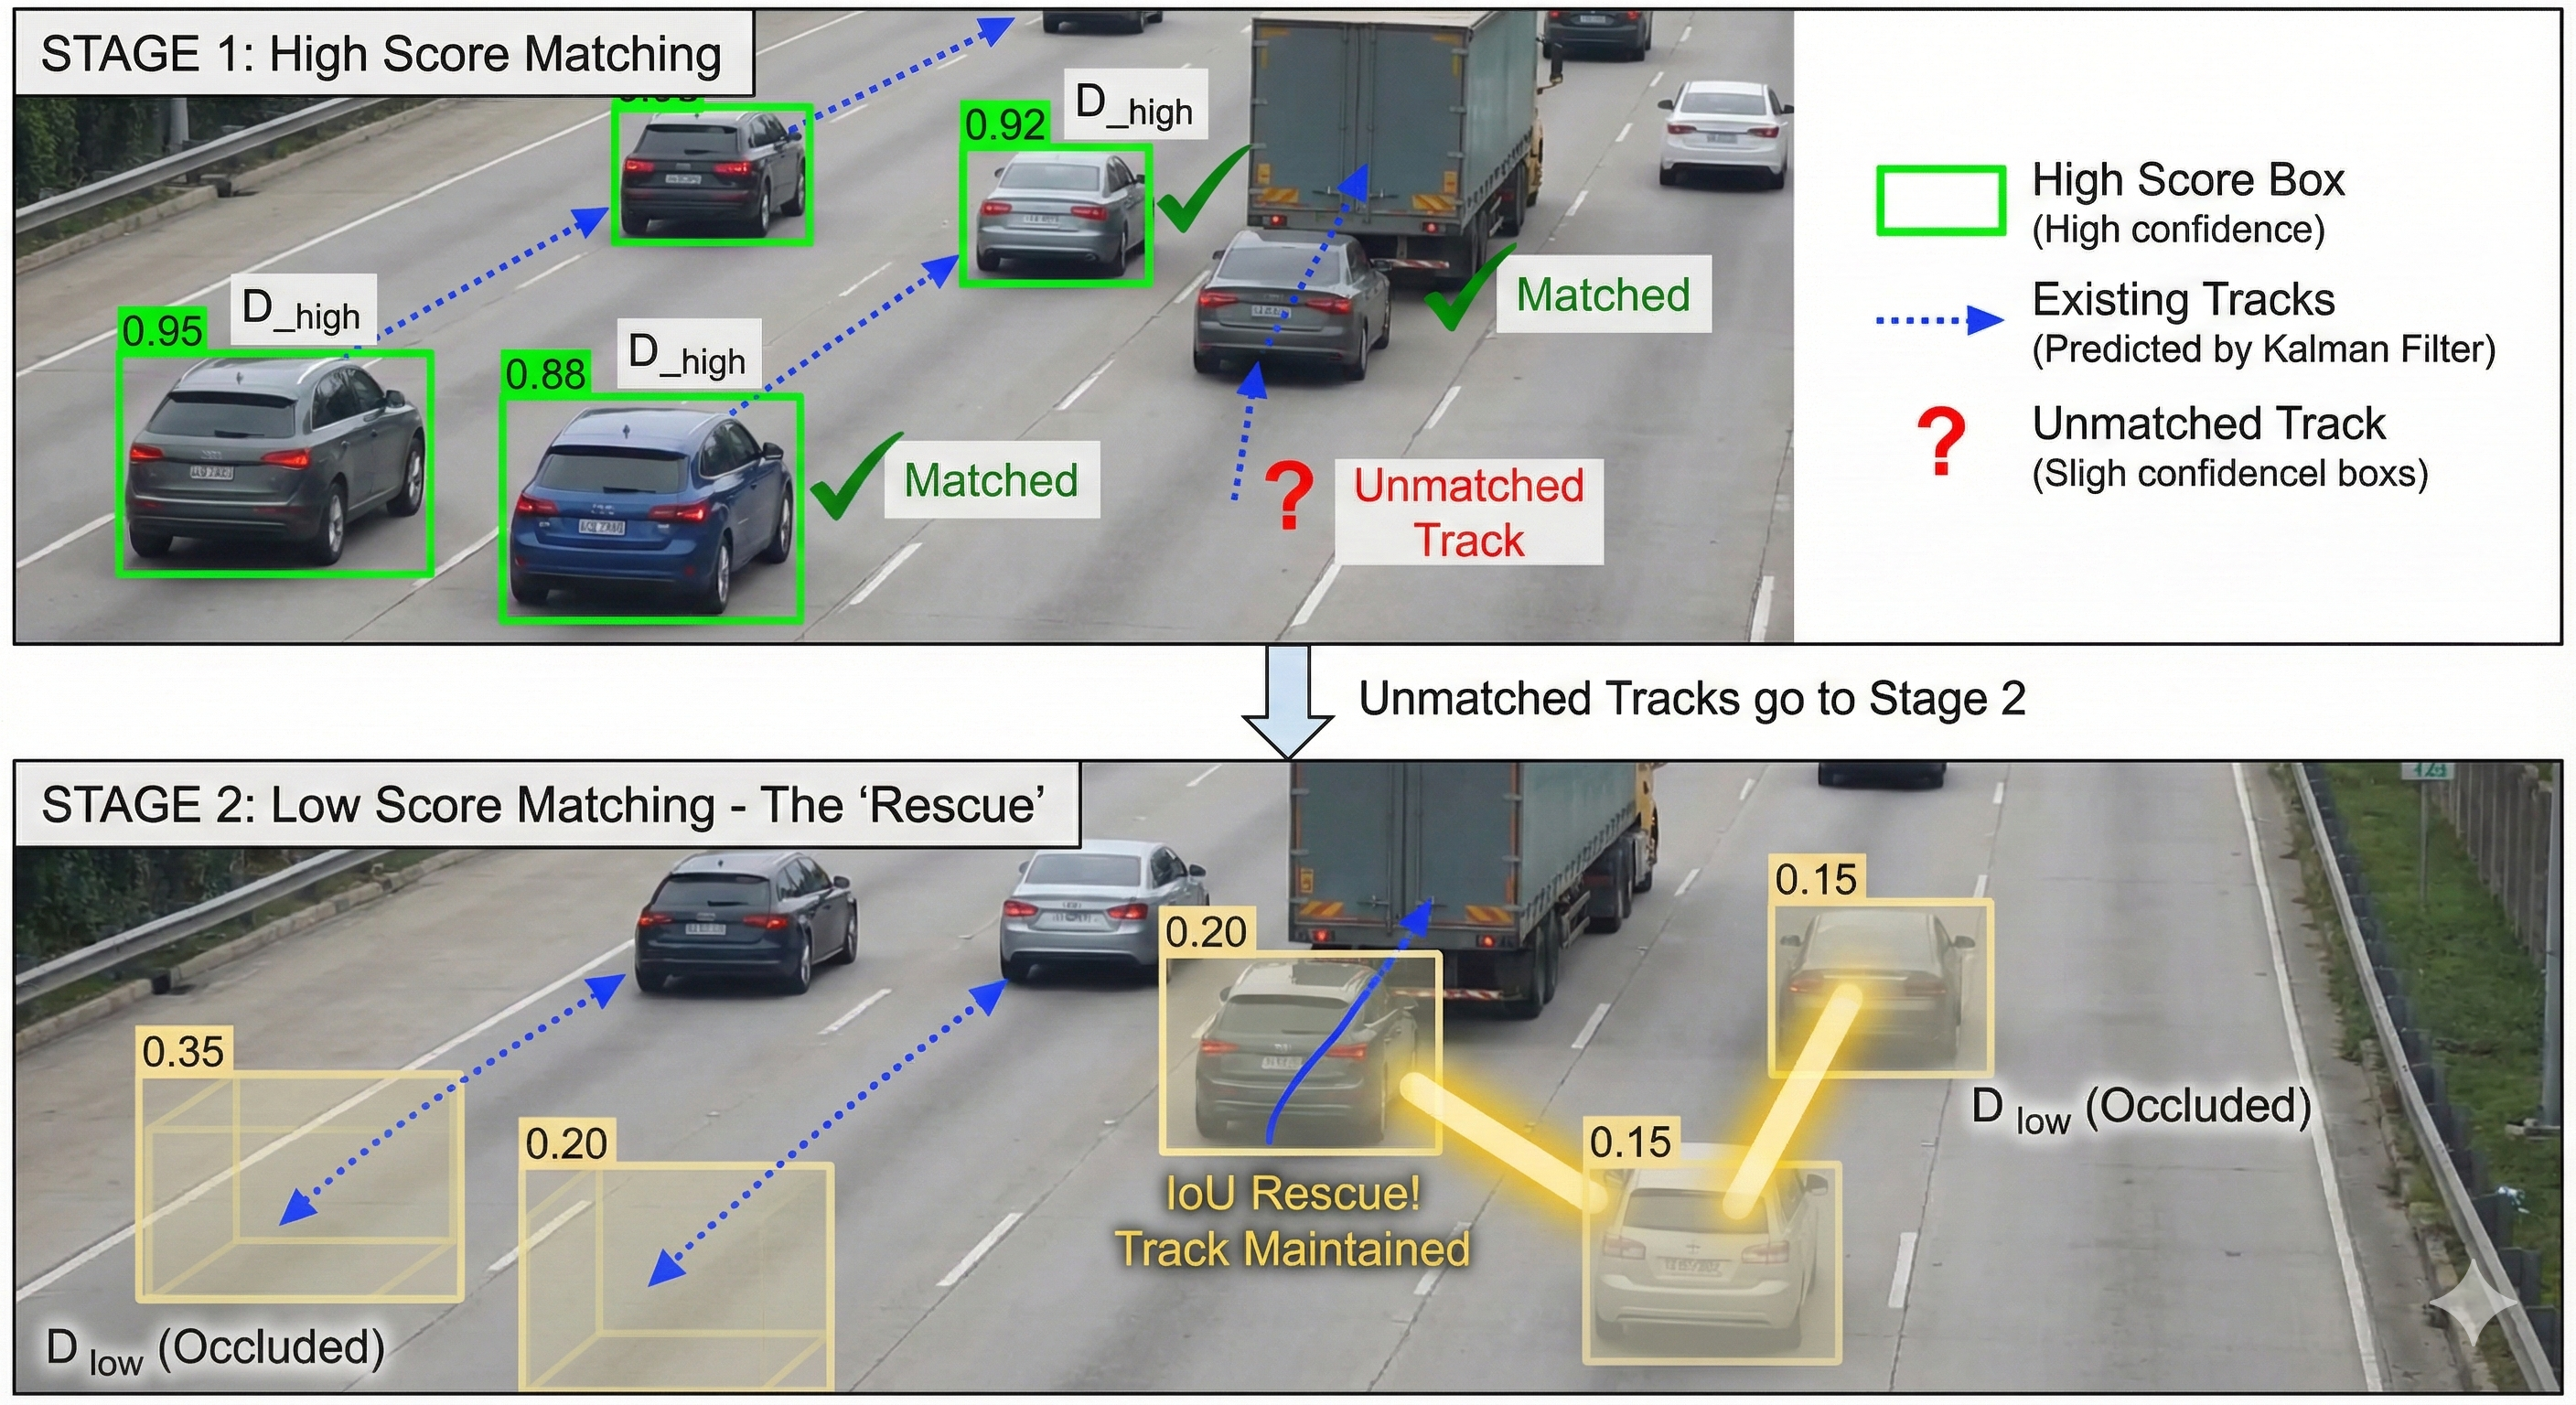
\includegraphics[width=0.8\linewidth]{Figures/bytetrack.png}
    \caption{Minh họa quy trình liên kết hai giai đoạn của ByteTrack}
    \label{fig:maching-bytrack}
\end{figure}

\subsubsection{Quản lý vòng đời Track}
\begin{itemize}
    \item \textbf{Track Birth (Sinh):} Các detection trong $\mathcal{D}_{high}$ không ghép được với bất kỳ track nào ở Giai đoạn 1 sẽ được xem là đối tượng mới xuất hiện và được cấp ID mới.
    \item \textbf{Track Death (Hủy):} Các Track không ghép được với bất kỳ detection nào (cả high và low) trong $K$ khung hình liên tiếp (ví dụ $K=30$) sẽ bị coi là đã ra khỏi khung hình và bị xóa bỏ.
\end{itemize}

\subsubsection{Ưu điểm đối với bài toán giao thông Việt Nam}
Việc áp dụng ByteTrack mang lại hai lợi ích lớn cho đề tài:
\begin{enumerate}
    \item \textbf{Xử lý che khuất:} Trong điều kiện giao thông hỗn hợp tại Việt Nam, xe máy thường xuyên bị xe buýt hoặc ô tô che khuất. ByteTrack giúp "gắp" lại các xe máy này ở giai đoạn 2, giảm thiểu việc đếm sai lưu lượng.
    \item \textbf{Giảm tải tính toán:} ByteTrack chỉ sử dụng thông tin hình học (geometric information) để liên kết mà không cần trích xuất đặc trưng ngoại hình (appearance features) bằng mạng nơ-ron sâu như DeepSORT. Điều này giúp giảm tải tính toán cho GPU và phù hợp triển khai thời gian thực.
\end{enumerate}

\section{Xử lý ảnh và Hình học tính toán}
\label{sec:cv_geometry}

Để giải quyết các bài toán cụ thể như nhận diện trạng thái đèn giao thông và xác định hành vi phương tiện (lấn làn, vượt đèn), hệ thống kết hợp các kỹ thuật xử lý ảnh trên không gian màu và các thuật toán hình học tính toán.

\subsection{Không gian màu HSV trong nhận diện tín hiệu đèn}
Chúng tôi chuyển đổi ảnh từ không gian màu RGB sang HSV để tách biệt thông tin màu sắc (Hue) khỏi độ sáng (Value), giúp thuật toán bền vững với thay đổi ánh sáng môi trường.

Quá trình chuyển đổi từ một điểm ảnh $(R, G, B)$ sang $(H, S, V)$ được thực hiện như sau. Đầu tiên, chuẩn hóa các giá trị $R, G, B \in [0, 1]$. Đặt $C_{max} = \max(R, G, B)$, $C_{min} = \min(R, G, B)$ và $\Delta = C_{max} - C_{min}$.

\begin{itemize}
    \item \textbf{Value (V):} Độ sáng của điểm ảnh.
    \begin{equation}
        V = C_{max}
    \end{equation}
    \item \textbf{Saturation (S):} Độ bão hòa màu.
    \begin{equation}
        S = \begin{cases}
            0 & \text{nếu } C_{max} = 0 \\
            \frac{\Delta}{C_{max}} & \text{nếu } C_{max} \neq 0
        \end{cases}
    \end{equation}
    \item \textbf{Hue (H):} Góc sắc độ (thể hiện màu sắc thuần túy).
    \begin{equation}
        H = \begin{cases}
            60^\circ \times (\frac{G - B}{\Delta} \mod 6) & \text{nếu } C_{max} = R \\
            60^\circ \times (\frac{B - R}{\Delta} + 2) & \text{nếu } C_{max} = G \\
            60^\circ \times (\frac{R - G}{\Delta} + 4) & \text{nếu } C_{max} = B
        \end{cases}
    \end{equation}
\end{itemize}

Hệ thống sử dụng các ngưỡng (threshold) trên kênh $H$ và $S$ để đếm số lượng pixel thuộc về màu Đỏ, Vàng, hoặc Xanh. Trạng thái đèn được xác định bởi màu có số lượng pixel vượt trội (dominant color).

\subsection{Hình học tính toán trong phát hiện vi phạm}

\subsubsection{Kiểm tra xe trong làn đường}
Làn đường là đa giác (không bắt buộc lồi) \(P = \{v_1,\dots,v_n\}\). Tâm xe \(C(x,y)\) được kiểm tra bằng hàm \texttt{cv2.pointPolygonTest} (tương đương ray casting): giá trị trả về \(\ge 0\) nếu điểm nằm trong/biên, \(<0\) nếu ngoài.

\subsubsection{Khoảng cách tới vạch dừng và sự kiện cắt qua}
Vạch dừng: đoạn \(P_1(x_1,y_1)\)--\(P_2(x_2,y_2)\). Khoảng cách vuông góc (đường thẳng qua \(P_1,P_2\)):
\[
d(C, P_1P_2) = \frac{|(x_2 - x_1)(y_1 - y_C) - (x_1 - x_C)(y_2 - y_1)|}{\sqrt{(x_2 - x_1)^2 + (y_2 - y_1)^2}}
\]
Trong code, khoảng cách được "kẹp" vào đoạn (nếu hình chiếu ra ngoài đoạn, lấy khoảng cách tới đầu mút).
Sự kiện vượt vạch khi: (i) \(d < \delta\) (mặc định 15--20 px), (ii) track ID chưa nằm trong tập xe đã qua vạch.

\subsubsection{Ước lượng hướng di chuyển dựa trên góc tham chiếu}
Hướng di chuyển đi thẳng được xác định bởi góc tham chiếu $\theta_{\text{ref}}$ (đơn vị: độ). Giá trị này mặc định là $90^\circ$ và được cập nhật khi hệ thống thiết lập Reference Vector.

Quá trình ước lượng dựa trên lịch sử vị trí bao gồm tối đa 10 điểm dữ liệu gần nhất. Để đảm bảo độ tin cậy, hệ thống yêu cầu tối thiểu 5 điểm dữ liệu và khoảng cách dịch chuyển phải lớn hơn 30 pixel. Từ vector chuyển động $\vec{v}=(dx, dy)$, góc di chuyển tuyệt đối $\theta$ và góc lệch tương đối $\theta_{\text{rel}}$ được tính toán như sau:
\[
    \theta = \operatorname{atan2}(dy, dx) \quad (\text{độ})
\]
\[
    \theta_{\text{rel}} = \theta - \theta_{\text{ref}}, \quad \text{với } \theta_{\text{rel}} \in [-180^\circ, 180^\circ]
\]

Phân loại hướng di chuyển với ngưỡng \(50^\circ\):
\[
\begin{cases}
\text{Đi thẳng} & |\theta_{\text{rel}}| \le 50^\circ \\
\text{Rẽ phải} & \theta_{\text{rel}} < -50^\circ \\
\text{Rẽ trái} & \theta_{\text{rel}} > 50^\circ
\end{cases}
\]

\textbf{Giải thích lựa chọn ngưỡng 50°:} Ngưỡng $50^\circ$ được chọn để phù hợp với đặc thù giao thông hỗn hợp nơi xe thường di chuyển theo nhiều hướng khác nhau tại các ngã tư. Ngưỡng này đủ rộng để hạn chế nhận diện sai các xe đi thẳng nhưng có độ lệch nhỏ do điều kiện đường sá, đồng thời đủ chặt để phân biệt rõ ràng giữa đi thẳng và rẽ.

% Minh họa vector tham chiếu vs. vector chuyển động
\begin{figure}[!htbp]
  \centering
  \begin{tikzpicture}[scale=1.6]
    \coordinate (O) at (0,0);
    % Reference vector (green) - hướng đi thẳng
    \draw[->,thick,green!70!black] (O) -- ++(90:2.2) node[above right] {$\vec r$ (ref - đi thẳng)};
    % Motion vector (red) - hướng xe đang đi
    \draw[->,thick,red] (O) -- ++(30:2.2) node[right] {$\vec v$ (xe)};
    % Angle arc showing relative angle
    \draw[->,orange,thick] (O) ++(90:0.9) arc (90:30:0.9);
    \node[orange] at (1.0,1.3) {$\theta_{\text{rel}}$};
    % Threshold lines at ±50°
    \draw[dashed,blue!60] (O) -- ++(140:2.0) node[left] {$+50^\circ$};
    \draw[dashed,blue!60] (O) -- ++(40:2.0) node[right] {$-50^\circ$};
    % Zone labels
    \node[green!50!black] at (-1,2.5) {\small Đi thẳng};
    \node[blue!70] at (-1.8,1.2) {\small Rẽ trái};
    \node[blue!70] at (1.8,0.5) {\small Rẽ phải};
    % Axes (faint)
    \draw[->,gray!40] (-0.3,0) -- (2.5,0) node[right] {$x$};
    \draw[->,gray!40] (0,-0.3) -- (0,2.8) node[above left] {$y$};
  \end{tikzpicture}
  \caption{So sánh góc chuyển động $\vec v$ với góc tham chiếu $\vec r$ (ngưỡng $50^\circ$). Vùng màu xanh lá: đi thẳng, vùng ngoài: rẽ trái/phải.}
  \label{fig:direction_reference}
\end{figure}
